%%
%% This is file `sample-sigconf.tex',
%% generated with the docstrip utility.
%%
%% The original source files were:
%%
%% samples.dtx  (with options: `sigconf')
%% 
%% IMPORTANT NOTICE:
%% 
%% For the copyright see the source file.
%% 
%% Any modified versions of this file must be renamed
%% with new filenames distinct from sample-sigconf.tex.
%% 
%% For distribution of the original source see the terms
%% for copying and modification in the file samples.dtx.
%% 
%% This generated file may be distributed as long as the
%% original source files, as listed above, are part of the
%% same distribution. (The sources need not necessarily be
%% in the same archive or directory.)
%%
%% The first command in your LaTeX source must be the \documentclass command.
\documentclass[sigconf]{acmart}
\usepackage[ruled,vlined,linesnumbered]{algorithm2e}
\usepackage{calc}
\usepackage{enumitem}
%% Rights management information.  This information is sent to you
%% when you complete the rights form.  These commands have SAMPLE
%% values in them; it is your responsibility as an author to replace
%% the commands and values with those provided to you when you
%% complete the rights form.
\setcopyright{acmcopyright}
\copyrightyear{2018}
\acmYear{2018}
\acmDOI{10.1145/1122445.1122456}

%% These commands are for a PROCEEDINGS abstract or paper.
\copyrightyear{2021}
\acmYear{2021}
\setcopyright{acmlicensed}\acmConference[SIGIR '21]{Proceedings of the 44th International ACM SIGIR Conference on Research and Development in Information Retrieval}{July 11--15, 2021}{Virtual Event, Canada}
\acmBooktitle{Proceedings of the 44th International ACM SIGIR Conference on Research and Development in Information Retrieval (SIGIR '21), July 11--15, 2021, Virtual Event, Canada}
\acmPrice{15.00}
\acmDOI{10.1145/3404835.3462791}
\acmISBN{978-1-4503-8037-9/21/07}

%%
%% Submission ID.
%% Use this when submitting an article to a sponsored event. You'll
%% receive a unique submission ID from the organizers
%% of the event, and this ID should be used as the parameter to this command.
%%\acmSubmissionID{123-A56-BU3}

%%
%% The majority of ACM publications use numbered citations and
%% references.  The command \citestyle{authoryear} switches to the
%% "author year" style.
%%
%% If you are preparing content for an event
%% sponsored by ACM SIGGRAPH, you must use the "author year" style of
%% citations and references.
%% Uncommenting
%% the next command will enable that style.
%%\citestyle{acmauthoryear}

%%
%% end of the preamble, start of the body of the document source.
\begin{document}

%%
%% The "title" command has an optional parameter,
%% allowing the author to define a "short title" to be used in page headers.
\title{PECAN: A Platform for Searching Chat Conversations}

%%
%% The "author" command and its associated commands are used to define
%% the authors and their affiliations.
%% Of note is the shared affiliation of the first two authors, and the
%% "authornote" and "authornotemark" commands
%% used to denote shared contribution to the research.
\author{Kunpeng Qin}
\email{kunpeng.qin@uq.net.au}
\affiliation{%
  \institution{The University of Queensland}
  \city{Brisbane}
  \country{Australia}
}
\author{Harrisen Scells}
\email{h.scells@uq.edu.au}
\affiliation{%
	\institution{The University of Queensland}
	\city{Brisbane}
	\country{Australia}
}

\author{Guido Zuccon}
\email{g.zuccons@uq.edu.au}
\affiliation{%
	\institution{The University of Queensland}
	\city{Brisbane}
	\country{Australia}
}

\newcommand{\todo}[1]{\textcolor{red}{#1}}

%%
%% The abstract is a short summary of the work to be presented in the
%% article.
\begin{abstract}
Often, existing chat services that organisations and individuals use today provide a way to search through previously sent messages. However, many of these chat services provide far-limited search functionalities, typically exact matching on individual messages. In this paper, we introduce a new task for addressing this problem, called \textit{searching for conversations}, whereby the aim is to retrieve and rank groups of related messages given a search query. We promote this task by providing a platform for research and development called PECAN. Our platform provides all the necessary functionality researchers need to conduct experiments on searching for conversations. Our system is also generic so as to support organisations and individuals who wish to search through their chat message archives.

We release PECAN to the wider community as an Open Source project available for download at \href{https://github.com/ielab/pecan}{https://github.com/ielab/pecan}.
\end{abstract}

%%
%% The code below is generated by the tool at http://dl.acm.org/ccs.cfm.
%% Please copy and paste the code instead of the example below.
%%
%\begin{CCSXML}
%<ccs2012>
% <concept>
%  <concept_id>10010520.10010553.10010562</concept_id>
%  <concept_desc>Computer systems organization~Embedded systems</concept_desc>
%  <concept_significance>500</concept_significance>
% </concept>
% <concept>
%  <concept_id>10010520.10010575.10010755</concept_id>
%  <concept_desc>Computer systems organization~Redundancy</concept_desc>
%  <concept_significance>300</concept_significance>
% </concept>
% <concept>
%  <concept_id>10010520.10010553.10010554</concept_id>
%  <concept_desc>Computer systems organization~Robotics</concept_desc>
%  <concept_significance>100</concept_significance>
% </concept>
% <concept>
%  <concept_id>10003033.10003083.10003095</concept_id>
%  <concept_desc>Networks~Network reliability</concept_desc>
%  <concept_significance>100</concept_significance>
% </concept>
%</ccs2012>
%\end{CCSXML}
%
%\ccsdesc[500]{Computer systems organization~Embedded systems}
%\ccsdesc[300]{Computer systems organization~Redundancy}
%\ccsdesc{Computer systems organization~Robotics}
%\ccsdesc[100]{Networks~Network reliability}

%%
%% Keywords. The author(s) should pick words that accurately describe
%% the work being presented. Separate the keywords with commas.
\keywords{search interface, chat search, searching for conversations}



%%
%% This command processes the author and affiliation and title
%% information and builds the first part of the formatted document.
\maketitle

\section{Problem, Target Users \& Importance}

Many search offerings of popular chat and messaging services of the likes of Slack, Discord, Signal, Whatsapp, etc., offer a sub-par experience: they mostly only allow exact matches between the user's query and their messages. However, this is not ideal because (1) the messages surrounding a targeted message often contain context to the information need, (2) semantic mismatch between the query and the messages severely impact retrieval quality. 
%. They mostly only allow searching for the exact messages that one might have in mind. 
%Existing message search systems are not ideal, as the messages surrounding a targeted message often contain context to the information need. 
An example of this is when searching for an answer to a question but not remembering how the question was posed. To find their answer, one may search for a conversation they knew that happened within the same time period. Indeed, within the context of chat message search, one is often not interested in individual messages relevant to a search query, but a \textit{conversation} of topically related messages. 
As search practitioners, we often want to understand how Information Retrieval systems work to improve them. Furthermore, we suggest that existing chat search systems can be drastically improved by addressing the task of `search for conversations' (rather than messages). In this new task, search within chat messages should not be restricted to individual messages and conversations of messages are the ideal unit of retrieval. To support researchers investigate and experiment with this task, we propose \textbf{PECAN}: A \textbf{P}latform for s\textbf{E}arching \textbf{C}h\textbf{A}t co\textbf{N}versations.

PECAN targets teams and organisations of chat services that wish to provide their own search solution and Information Retrieval practitioners that wish to study how users search for conversations and improve the effectiveness of searching for conversation. PECAN provides all of the necessary tools to get started working on this task: a componentised framework, which can be further enhanced through the upgrade or implementation of new features, offline/batch retrieval for evaluation, and user study instrumentation (administration, query logging, interaction logging). An overview of PECAN's features and architecture  is presented in Figure~\ref{fig:overview}.
 
\begin{figure}
	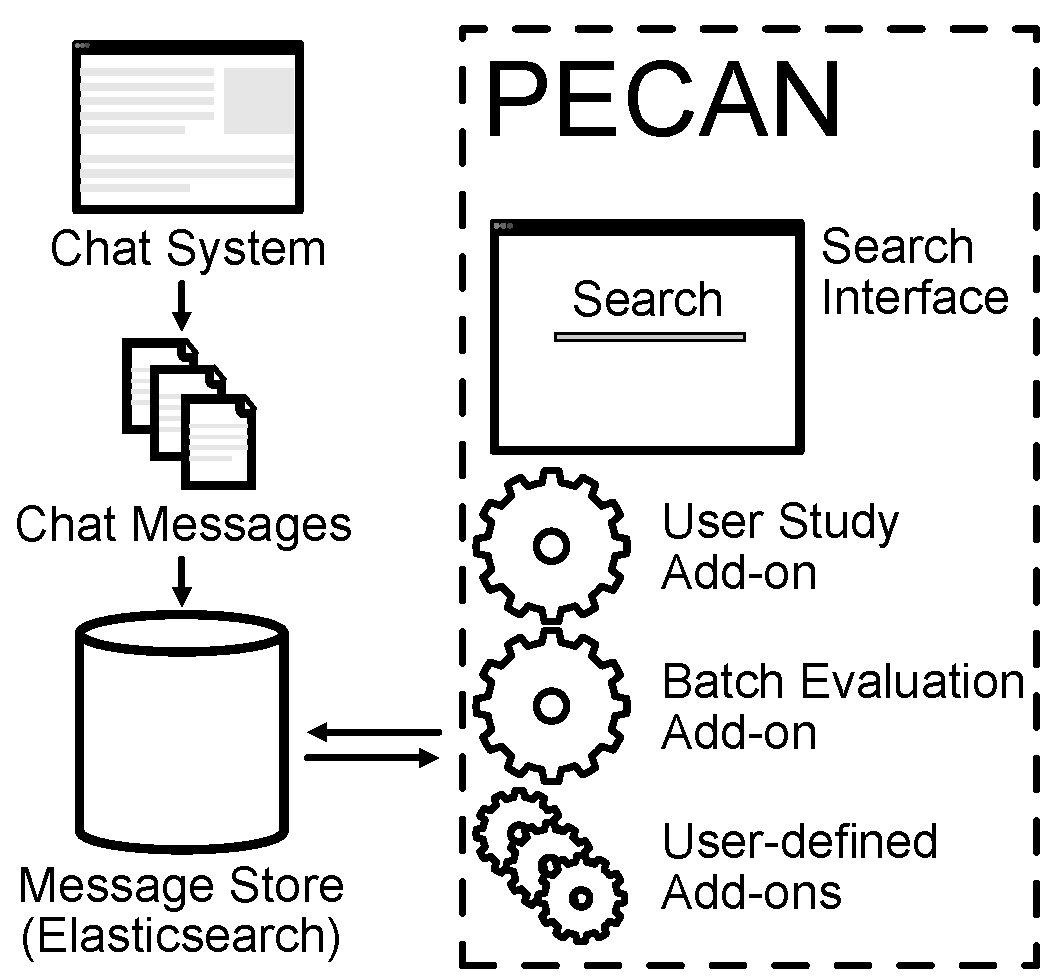
\includegraphics[width=\linewidth]{overview}
	\caption{Overview of the architecture of the PECAN system.\vspace{-16pt}}
	\label{fig:overview}
\end{figure} 
 
\section{Importance of System}

To the best of our knowledge, PECAN is the only system currently available to enable research into this new task of `searching for conversations'. There are many facets to this new research task that PECAN can be used for implementing new algorithms:

\begin{description}
\item[Conversation Aggregations:] The challenge involved here is how to represent the `unit of retrieval'. Two aggregation aspects can be addressed: Message Relevance and Conversation Boundaries. Message Relevance is the task of identifying which messages within a conversation are relevant and possibly discarding irrelevant messages from the presentation of the results. Conversation Boundaries is the task of identifying when a conversation begins and ends and merging retrieved conversations that overlap in time or topic.
\item[Conversation Scoring:] This is the task of scoring conversations given a query to provide a ranking of conversations in terms of relevance, for example. It is currently an open question for the most effective way to rank conversations and may depend on various factors from typical search scenarios, such as timeliness.
\item[Query Suggestion:] This is the task of suggesting alternative queries for searching conversations. We hypothesise that most searches for conversations are known-item retrieval (e.g., a user is searching to find an answer to a question they previously had but cannot remember how the question was asked or the answer). This scenario presents itself as a unique opportunity to apply query suggestion to known-item retrieval.
\item[Conversation Summarisation:] Conversations are rich sources of information that contain the history of questions and answers asked by a team or organisation. However, finding answers to complex questions within conversations can be tedious as one may need to read through many messages to find the answer. This task aims to summarise conversations to provide an answer to a question or a high-level overview of a conversation.
\item[Related Conversations:] This is the task of identifying similar conversations given a conversation. This task is useful in the case of, for example, showing that a topic of conversation has been discussed previously (i.e., preventing time-wasting, keeping track of important decisions).
\end{description}
 
 
\graphicspath{ {./images/} }
\section{Operation of the System}

\subsection{Searching for Conversations}

\todo{1st priority: for @kq: use images to describe how a user uses the system. each image has a caption, in the text expand upon the caption. give a "fake" case study, the user first enters a query, then they look through conversations, then they do blah... etc.}

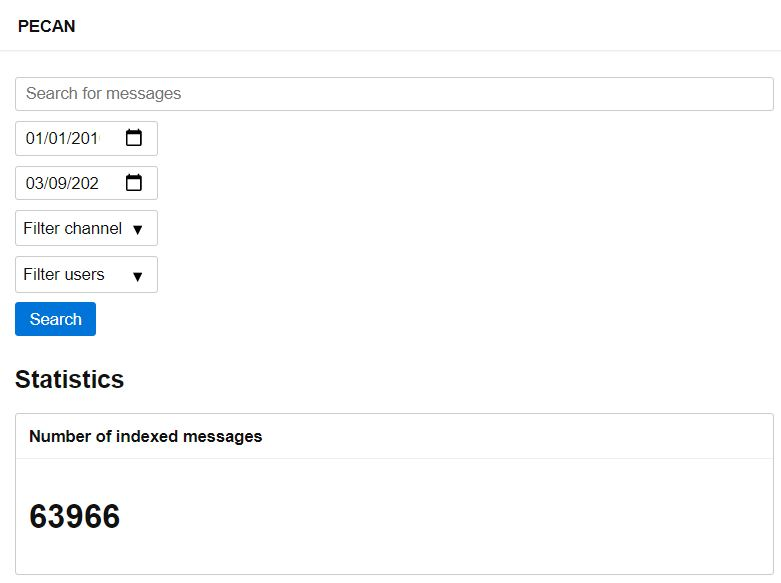
\includegraphics[scale=0.2]{homepage}

This is the homepage of the system.
\bigbreak

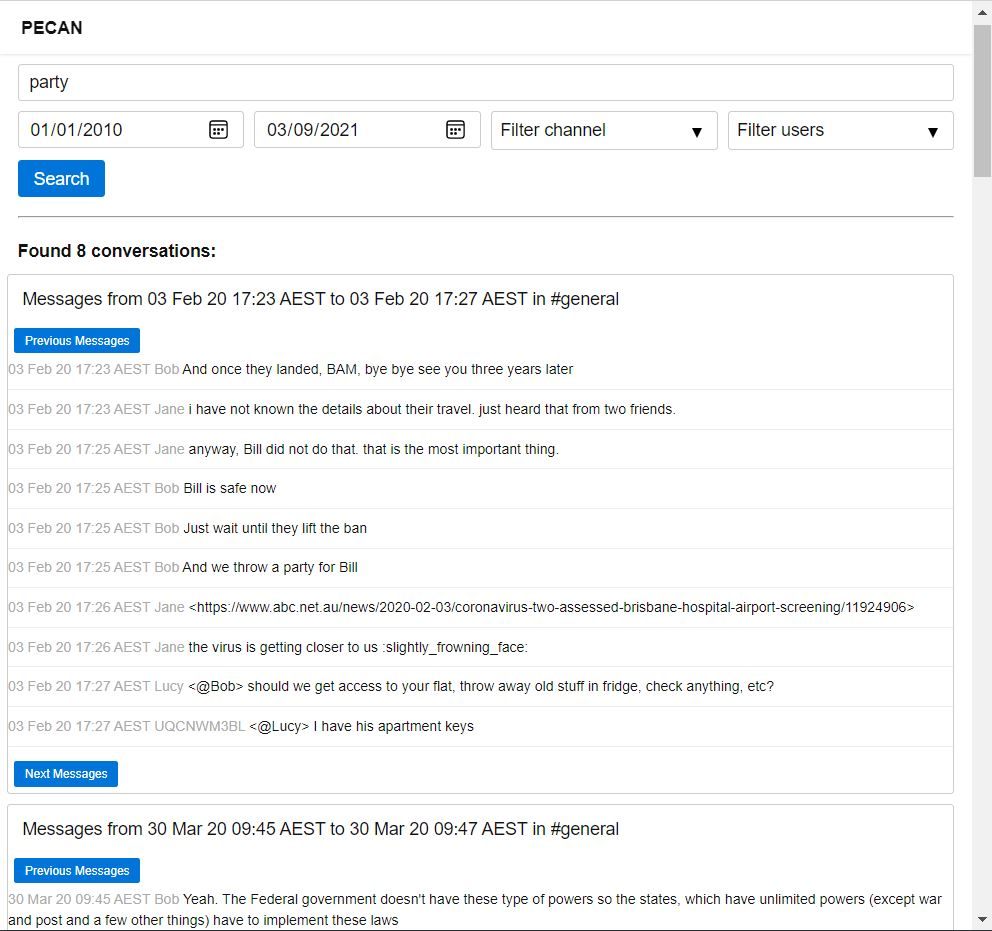
\includegraphics[scale=0.2]{searching}

Searching for converstaions with query "party".
\bigbreak

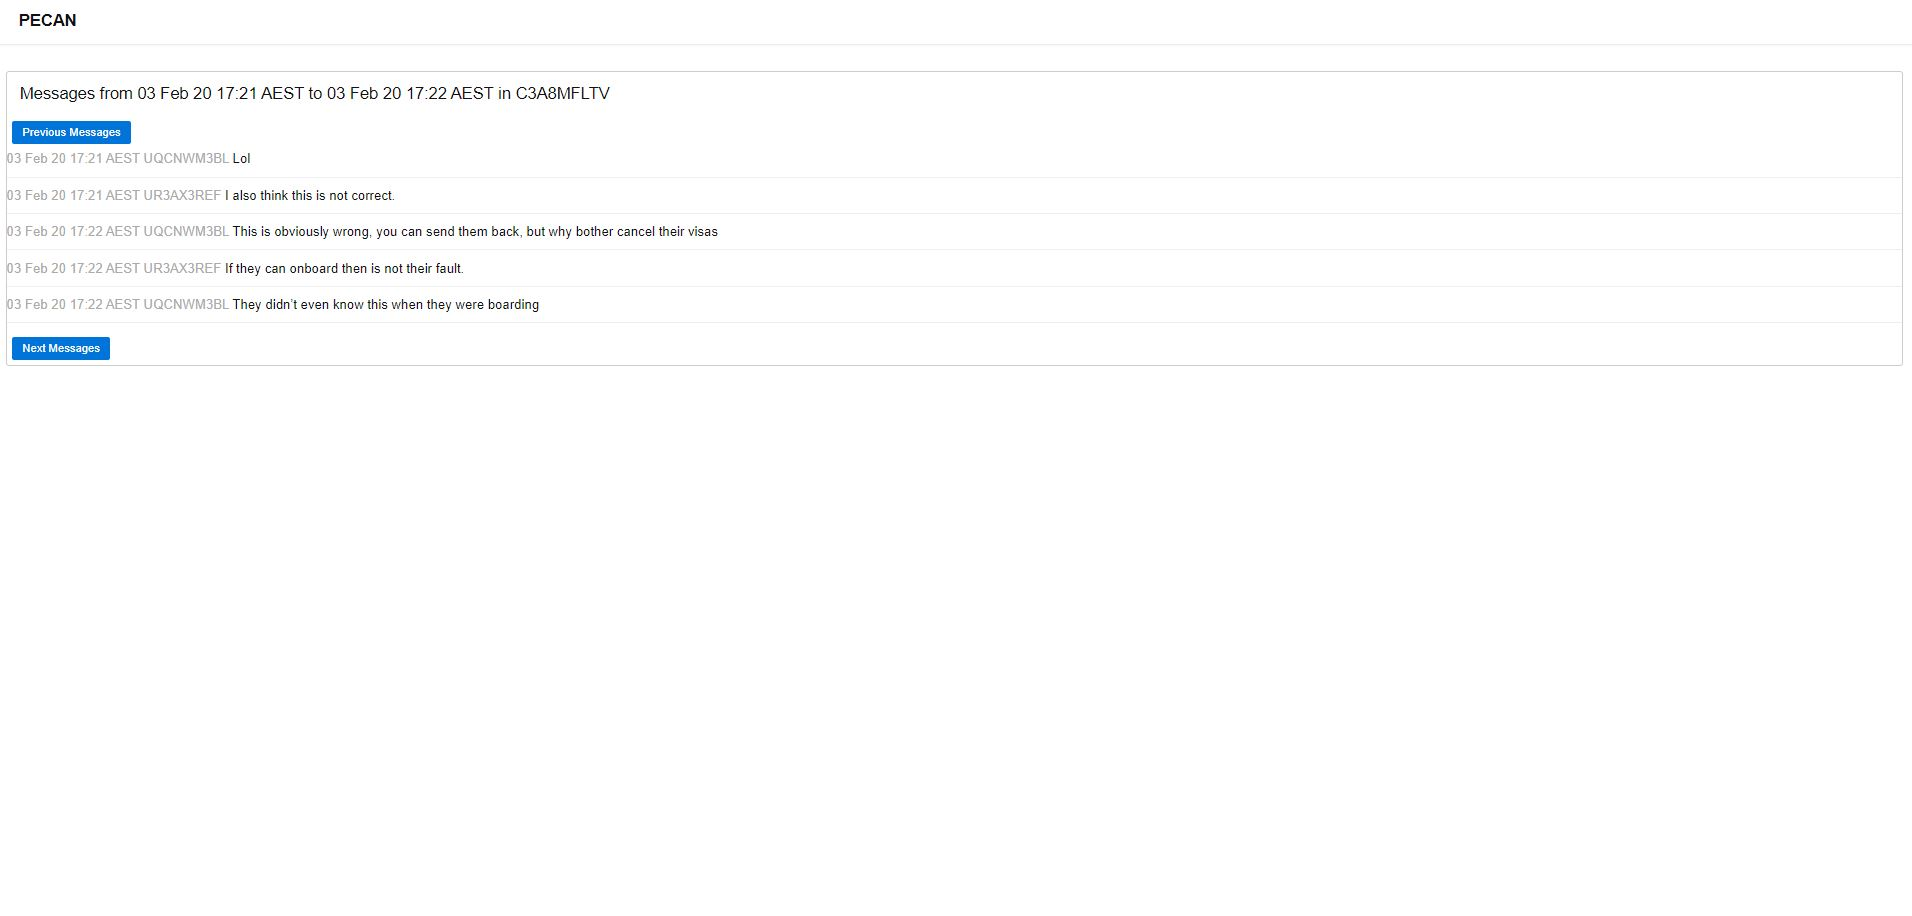
\includegraphics[scale=0.2]{traversing}

Traversing previous or next messages by clicking "previous messages" or "next messages".
\bigbreak

\subsection{System Implementation}
In this project, we use Go Language to implement the backend part of the system. We use elastic 7.0 as our serach engine. The elastic search provides a go module so that we can import and use it. The retrieval model we use to score messages is BM25. The score of each conversation is simply the sum of the scores of messages in that conversation. The retrieved conversations are merged and than ranked based on their scores. Users can access the system by searching with queries through an interface. The system will return conversations that are related to the query. After getting all the conversations, users can traversing through messages that come before and after each conversation.

\subsubsection{Conversation Aggregation}
There are many ways to retrieve conversations instead of messages. In this project we find conversations based on original messages. When we get a message, we define the five nearest messages before this message and five nearest messages after this message to be in the same conversation with this target message. We can retrieve these messages very easily with elastic search. These messages are then combined as one conversation. After retrieving all the conversations we want, we merge conversations that have identical messages. After merging conversations, we rank them by the sum of the scores of messages they have using quicksort. Normally, merged conversations are ranked higher than original conversations. Below is the pseudocode of the algorithm.

\begin{algorithm}
	\SetAlgoLined
	\caption{Retrieve Conversations}
	\SetKwInOut{Input}{inputs}
	\SetKwInOut{Output}{output}
	\SetKwProg{CreateConversations}{CreateConversations}{}{}
	\CreateConversations{$(Messages)$}{
		\Input{$messages$}
		\Output{$conversations$}
		$conversations \gets []$\\
		$i \gets 0$\\
		\ForEach{$message \in messages$}{
			$conversation \gets getSurroundingMessages(message$)\\
			$conversations[i] \gets conversation$\\
		}
		\Return{rankConversations(mergeConversations($conversations$))}
	}
\end{algorithm}
		
\subsubsection{Conversation Scoring}

\todo{3rd priority: for @kq: describe algorithms: mergeConversations, rankConversations}
To merge the conversations we retrieved, we simply go through every conversation. Since different conversations may have different channels, we keep an index for each channel so that we don't merge conversations with different channels together. We store the merged conversations into an array and for each channel, we save the index of the last conversation of the same channel in a map. Therefore, for each conversation, we can look for it's previous conversation with the same channel and check if they are overlapped. If they are overlapped we merge them and replace the old conversation on the index with the new conversation. Otherwise we insert the new conversation into the array and update the index for that channel.

\begin{algorithm}
	\SetAlgoLined
	\caption{Merge Conversations}
	\SetKwInOut{Input}{inputs}
	\SetKwInOut{Output}{output}
	\SetKwProg{MergeConversations}{MergeConversations}{}{}
	\MergeConversations{$(Messages)$}{
		\Input{$conversations$}
		\Output{$C$}
		$C \gets []$\\
		$H \gets HashMap$\\
		\ForEach{$conversation \in conversations$}{
			$index \gets H.get(conversation[0].Channel)$\\
			\If{$index \neq null$ and $conversation[0].Timestamp >= 	C[index][len(C[index])-1].Timestamp$}{
				\ForEach{$message \in conversation$}{
					\If{$message.Timestamp < C[index][len(C[index])-1].Timestamp$}{
							$C[index].append(message)$
					}
					\ElseIf{$message.Score>0$}{
						\ForEach{$keyMessage \in C[index]$}{
							\If{$keyMessage.Timestamp == message.Timestamp$ AND $keyMessage.Text==message.Text$}{
									$keyMessage \gets message$
							}
						}
					}
				}
			}
			\Else{
				$C.append(conversation)$
				$H[conversation[0].Channel] = len(C) -1$
			}
		}
		\Return{$C$}
	}
\end{algorithm}


\subsection{Running a User Study}

\todo{for @hs: description for how to use PECAN in a user study, how to use query logging, interaction logging.}

\subsection{Batch Evaluation}

\todo{for @hs}

\subsection{Planned Features}

\todo{4th priority: for @kq: channel filtering (in search time), filter by author, attachment search}
\section{Comparison with Existing Systems}

In our survey of the literature, we found no such research for the explicit task of searching for conversations. More so, we did not identify any such research-oriented systems for searching chat conversations, or messages for that matter. However, in terms of the research tasks related to searching for conversations put forward in Section~\ref{sec:importance}, we have identified a number of works that have addressed these tasks, and would have benefited from the PECAN ecosystem.

For the task of conversation scoring, Magnani et al.~\cite{magnani2012conversation} propose a conversation ranking framework for micro-blogging (e.g., Twitter). For this task, there are many signals of relevance that do not exist in our task, for example, popularity metrics such as likes. This task also models conversations with explicit replies to posts. Our task differs in that multiple, different, overlapping conversations may occur all at the same time.

In terms of conversation aggregation, Khan et al.~\cite{khan2002mining} identify this as a problem for studying tasks involving chat messages and propose a rule-based classification system to detect when conversations begin and end. However, their results highlight that rule-based methods are not scalable, especially in multi-lingual contexts. Shen et al.~\cite{shen2006thread} takes a different approach and instead attempt to detect topically related conversations in chat messages using a novel single-pass clustering algorithm. Such methods are possible to be implemented directly into PECAN, allowing research into this task.

While we did not identify any works on query suggestion for chat messages or chat conversations, we did identify research in related domains. For example, Mishne et al.~\cite{mishne2013fast} present an architecture of Twitter's real-time related query suggestion, where relevance signals from query logs are used to suggest related queries to users. Carmel et al.~\cite{carmel2017demographics} investigate demographical applications to query suggestion in email search, where one could consider similarities between email and chat messages. Their results indicate that personalisation is important for suggesting effective queries. PECAN's query logging may be used to capture data related to these works, allowing research into this task.

For the task of conversation summarisation, Bengel et al.~\cite{bengel2004chattrack} propose an interface for intelligence agencies to monitor chat participants that can identify latent topics of conversations in channels or of individual users. They also provide a basic interface that allows agents to search for messages. Our idea of conversation summarisation differs from this in that we seek to provide a succinct summary of the conversation that took place, rather than trying to classify the topics of a conversation. 

\section{Impact of the System}


%%
%% The acknowledgments section is defined using the "acks" environment
%% (and NOT an unnumbered section). This ensures the proper
%% identification of the section in the article metadata, and the
%% consistent spelling of the heading.
%\begin{acks}
\small
\subsubsection*{Acknowledgements}
Dr Guido Zuccon is the recipient of an Australian Research Council DECRA Research Fellowship (DE180101579) and Google Faculty Award.
%\end{acks}

%%
%% The next two lines define the bibliography style to be used, and
%% the bibliography file.
\bibliographystyle{ACM-Reference-Format}
\bibliography{bibliography}

%%
%% If your work has an appendix, this is the place to put it.
\appendix

\end{document}
\endinput
%%
%% End of file `sample-sigconf.tex'.
